\documentclass[report]{BetterDocument}

\newcommand{\bdd}{base de données}

\title{Équida}
\subtitle{Mise en production}
\who{MARTIN Justine\\
	BOTTON Léa}
\date{2019}
\place{BTS SIO 2 - Jean Rostand Caen - E4}

\begin{document}

	\pageDeGarde

	\chapter{Procédure}

		On se connecte au serveur en utilisant les identifiants fournis dans \nameref{sec:ressources}.

		On va commencer par cloner le projet dans le home de root. En étant connecté en tant que root on fait donc :

		\begin{itemize}
			\item{cd}
			\item{git clone https://github.com/justine-martin-study/Equida}
		\end{itemize}

		On va ensuite installer phpmyadmin, php, mysql, apache2 afin de pouvoir gérer la base de données de manière graphique grâce à PhpMyAdmin.

		\begin{figure}[H]
			\centering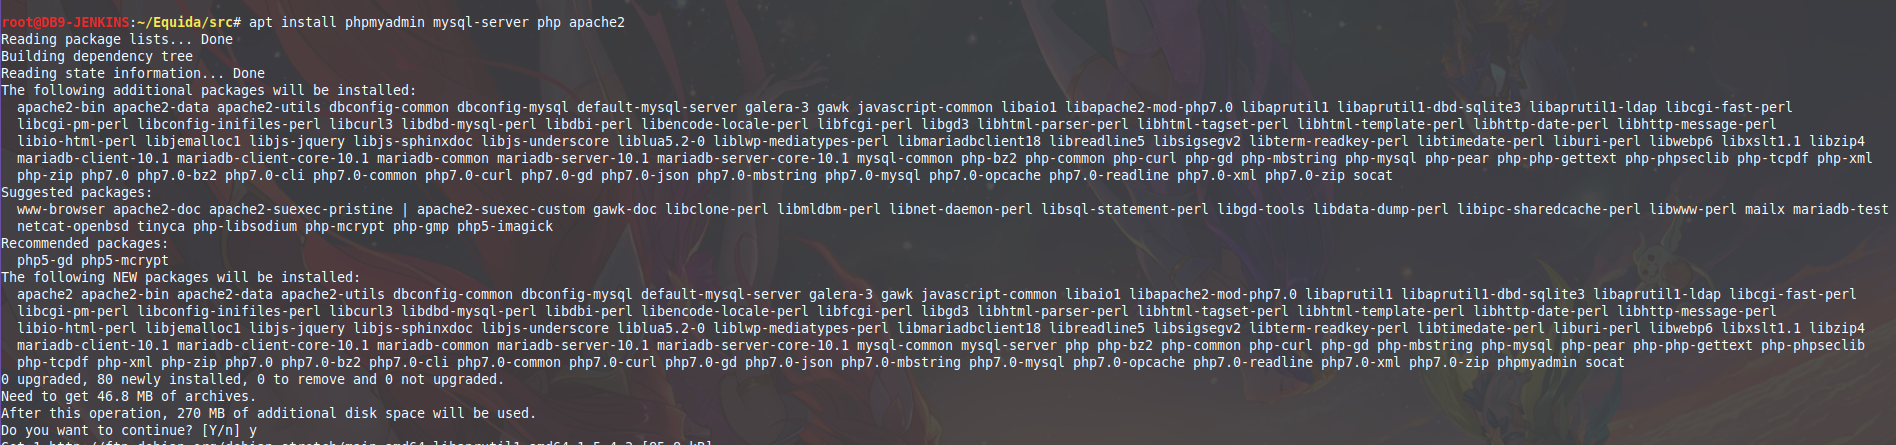
\includegraphics[width=0.85\textwidth, keepaspectratio]{res/install-lampp.png}
			\caption{Installation de lampp}
		\end{figure}

		Il faut maintenant autoriser l'utilisateur phpmyadmin à se connecter à la \bdd{}. Ainsi, on va se connecter à la \bdd{} en utilisant la commande mysql.

		\begin{itemize}
			\item{mysql -u root -p}
		\end{itemize}

		Après avoir saisi le mot de passe choisi à l'installation, on arrive sur l'invite de commande du serveur MySql. Sur cette console il faut alors taper les commandes suivantes :

		\begin{itemize}
			\item{GRANT ALL PRIVILEGES ON *.* TO 'phpmyadmin'@'localhost';}
			\item{FLUSH PRIVILEGES;}
			\item{EXIT}
		\end{itemize}

		On peut maintenant éxécuter les scripts SQL du dépot Git par l'intermédiaire de PhpMyAdmin. On crée alors la \bdd{} "equida" et on y éxécute les scripts SQL.

		\begin{figure}[H]
			\centering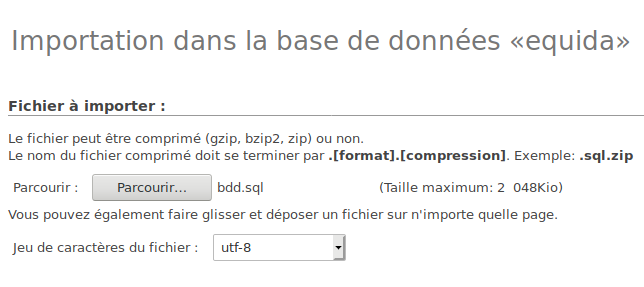
\includegraphics[width=0.55\textwidth, keepaspectratio]{res/sql-bdd.png}
			\caption{Exécution des scripts SQL}
		\end{figure}

		\textit{NB : Tous les scripts ont auparavant été compilés en 1 seul nommé bdd.sql}

		On obtient alors la \bdd{} avec toutes ses tables et ses enregistrements.

		\begin{figure}[H]
			\centering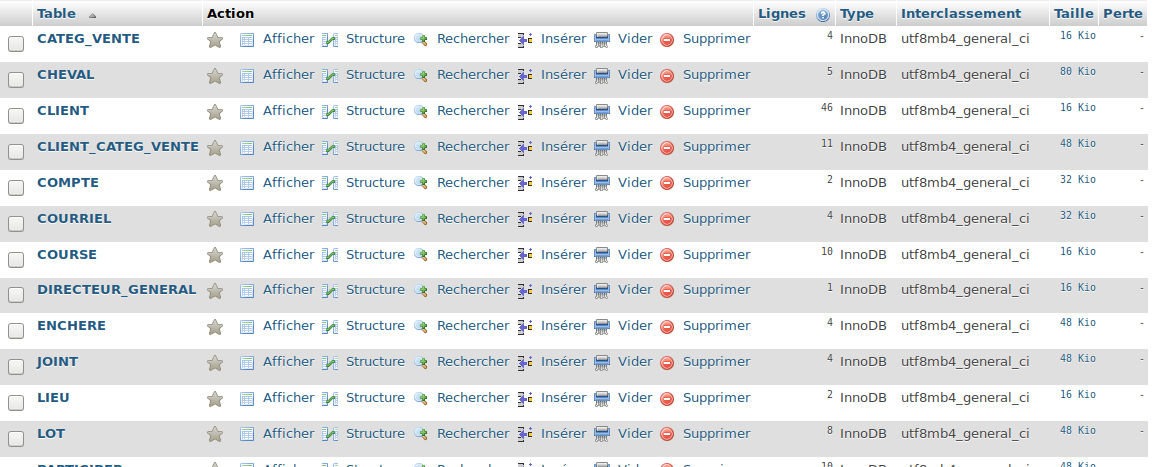
\includegraphics[width=0.75\textwidth, keepaspectratio]{res/bdd.png}
			\caption{\bdd{} Post éxécution des script SQL}
		\end{figure}

		Maintenant que la \bdd{} est fonctionnelle, on doit permettre le lancement des applications développées. On va donc installer nodejs (et npm). Java 8 étant déjà présent par défaut, il n'est pas nécessaire de le préciser dans la commande. Sur notre version de Debian, NodeJs n'était pas fourni dans une version suffisamment haute pour faire fonctionner ionic. On a donc du ajouter le dépot de ionic à la liste des dépots utilisés.

		\begin{itemize}
			\item{apt install curl}
			\item{curl -sL https://deb.nodesource.com/setup\_8.x | bash -}
 			\item{apt install nodejs npm}
			\item{npm install -g ionic}
		\end{itemize}

		\begin{figure}[H]
			\centering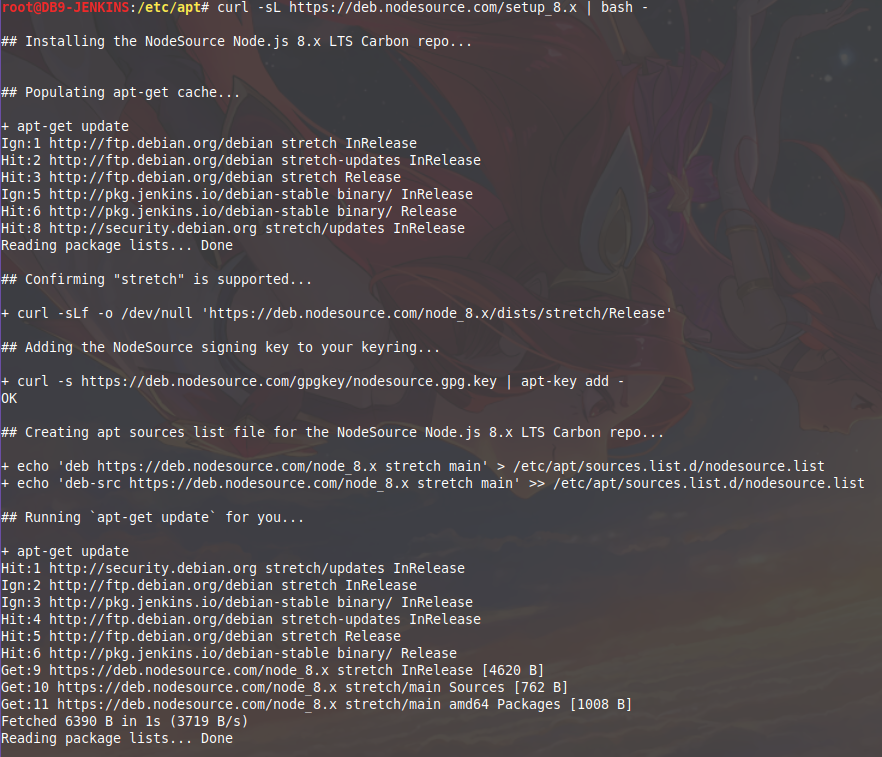
\includegraphics[width=0.75\textwidth, keepaspectratio]{res/install-npm.png}
			\caption{Ajout du dépot officiel de NodeJs}
		\end{figure}

		Pour compiler les projets basés sur Spring Boot, on doit installer Gradle sur le serveur.

		\begin{itemize}
			\item{cd /tmp}
			\item{wget https://services.gradle.org/distributions/gradle-5.4.1-all.zip}
 			\item{mkdir /opt/gradle}
			\item{unzip -d /opt/gradle gradle-5.4.1-all.zip}
		\end{itemize}

		Pour que l'on puisse utiliser la commande "gradle", il faut modifier le .bashrc de root et y ajouter cette ligne :
		export PATH=\$PATH:/opt/gradle/gradle-5.4.1/bin

		\begin{figure}[H]
			\centering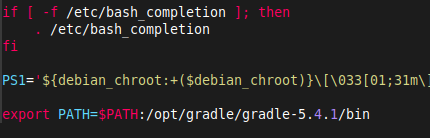
\includegraphics[width=0.5\textwidth, keepaspectratio]{res/bashrc-path.png}
			\caption{Modification du PATH dans le .bashrc}
		\end{figure}

		Afin de prendre en compte les changements, on se déconnecte puis on se reconnecte en tant que root.

		Nous créons des services pour gérer plus efficacement le lancement automatique des applications lors d'un démarage ou après un redémarrage en cas d'interruption lors d'un crash par exemple, etc. Les services ajoutés sont donc equidaIonic pour démarrer le projet Ionic, equidaRest pour démarrer l'API, equidaWebApp pour démarrer le site web. On a donc le code suivant pour les services :

		\begin{figure}[H]
			\centering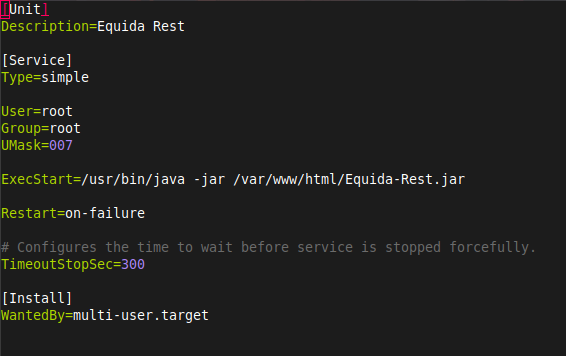
\includegraphics[width=0.65\textwidth, keepaspectratio]{res/service-equidaRest.png}
			\caption{Service equidaRest}
		\end{figure}

		\begin{figure}[H]
			\centering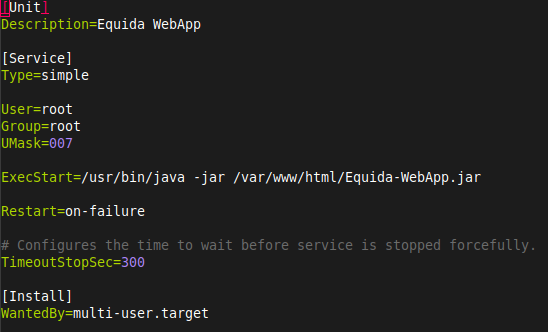
\includegraphics[width=0.65\textwidth, keepaspectratio]{res/service-equidaWebApp.png}
			\caption{Service equidaWebApp}
		\end{figure}

		\begin{figure}[H]
			\centering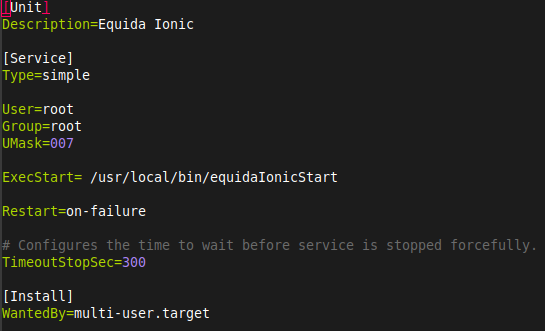
\includegraphics[width=0.65\textwidth, keepaspectratio]{res/service-equidaIonic.png}
			\caption{Service equidaIonic}
		\end{figure}

		Le script equidaIonicStart est le suivant :

		\begin{figure}[H]
			\centering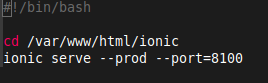
\includegraphics[width=0.4\textwidth, keepaspectratio]{res/script-equidaIonicStart.png}
			\caption{Script equidaIonicStart}
		\end{figure}

		Ce script est situé dans /usr/local/bin et est bien entendu éxécutable.

		Afin d'automatiser la mise en production des applications, un script "updateEquida" est créé. Voici son code :

		\begin{figure}[H]
			\centering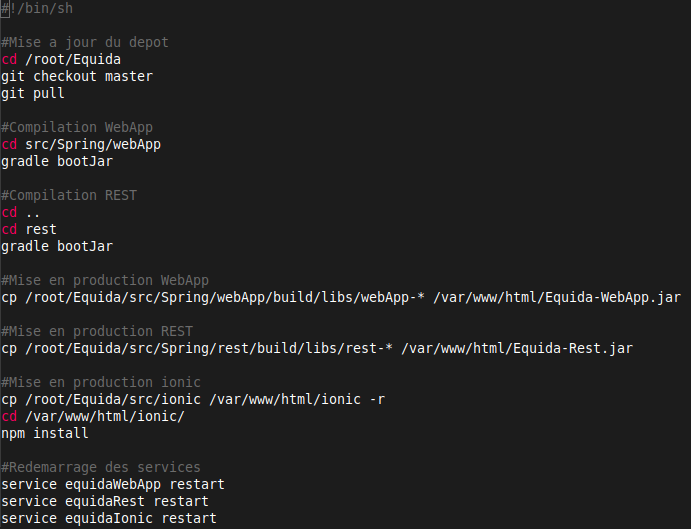
\includegraphics[width=0.75\textwidth, keepaspectratio]{res/script-updateEquida.png}
			\caption{Script updateEquida}
		\end{figure}

		Ce script est également situé dans /usr/local/bin et est éxécutable lui aussi.

	\chapter{Gestion des applications}

		La gestion des applications est donc simplifiée. On peut gérer leur éxécution avec l'utilisation de la commande "service" ou "systemctl".

		Concernant la mise à jour des applications en production, il suffit d'éxécuter la commande "updateEquida" qui va alors pull la branche master, car c'est celle qui est considérée comme étant stable, puis remplacer les anciennes applications par les nouvelles fraichement compilées. Cependant, il est très important de noter que le script ne permet pas de modifier la ligne de la classe "rest-api.service" qui indiqe l'url de l'api Rest dans le projet Ionic. il faut donc modifier manuellement cette ligne pour le moment.

	\chapter{Ressources}
		\label{sec:ressources}
		\noindent
		Accès serveur en local (ssh) : 172.20.0.249:22\\
		Accès serveur à distance (ssh) : nas.inforostand14.net:2249\\
		Compte utilisateur : leaju/mpLeaju\\
		Compte Admin : root/adm5RV\\
		Compte BDD : phpmyadmin/mpLeaju

\end{document}

% Aide pour la prise en main de Latex.
% Les lignes qui commencent par "%" sont des commentaires.

% =========================

% Structurer un document

% Dans l'ordre on retrouve les éléments suivants :

% \part{part name}
% \chapter{chapter name}
% \section{section name}
% \subsection{subsection name}
% \subsubsection{subsubsection name}

% =========================

% Afficher une image

%	\begin{figure}[H]
%		\centering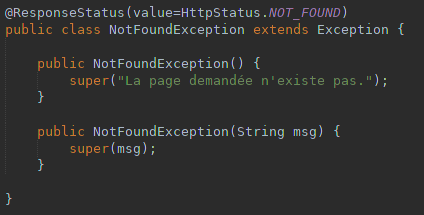
\includegraphics[width=0.75\textwidth, keepaspectratio]{res/NotFoundException.png}
%		\caption{Code de NotFoundException}
%	\end{figure}

% caption permet d'afficher une légende
% width permet de définir la taille en largeur de l'image par rapport à la taille de la feuille (ici 75%)
% res/NotFoundException.png -> Nom de l'image

% =========================

% Faire une liste à points

%	Blablabla, ainsi on peut citer :
%	\begin{itemize}
%		\item{signaler une erreur}
%		\item{mieux gérer les ...}
%	\end{itemize}

% =========================

% Faire une liste descriptive

%	Blablabla, on a donc les éléments suivants :
%	\begin{description}
%		\item[Service]{Fait l'intermédiaire entre ...}
%		\item[Repository]{Permet de faire ...}
%	\end{description}
